% Chapter 1: Introduction (revised version, thesis_v2)
\chapter{Introduction}\label{chap:introduction}

\section{Background and Motivation}

Automatic readability assessment estimates how difficult a text is for a given group of
readers. It is an established research topic in Natural Language Processing (NLP) and in
educational technology \cite{dubay2004principles,collins2014computational}, and it is used to
choose reading material for learners, to design curricula, to support intelligent tutoring
systems and to guide and evaluate text simplification \cite{vajjala2022trends}. The field
started with readability formulas built on sentence and word length
\cite{flesch1948readability,dale1948formula}, moved to machine learning over hand-crafted
linguistic features \cite{schwarm2005reading}, and is now dominated by pretrained transformer
models \cite{martinc2021supervised,deutsch2020linguistic}.

Most of that history was written for English. Arabic has received far less attention and is
harder to model, because of its rich morphology, its clitics, the usual absence of short
vowels in writing, and its lexical ambiguity \cite{nassiri2023approaches}. Before 2025, Arabic
readability work relied on formulas adapted from English
\cite{al2010automatic,altamimi2014aari,elhaj2016osman}, on feature-based classifiers trained on
school or learner material with three to five levels
\cite{saddiki2018feature,khallaf2021automatic}, and on resources such as the SAMER readability
lexicon \cite{alkhalil2020samer}, the SAMER simplification corpus \cite{alhafni2024samer} and
the DARES dataset of Saudi school textbooks \cite{elhaj2024dares}. Each of these made progress,
but none offered a large, openly split, sentence-level corpus with a fine-grained scale on which
different models could be compared, which Chapter~\ref{chap:relatedwork} examines in detail.

The Balanced Arabic Readability Evaluation Corpus (BAREC) filled that gap
\cite{elmadani2025barec}. It contains 69{,}441 sentences annotated on 19 readability levels,
named in the Abjad order of the Arabic letters (1-\textit{alif} to 19-\textit{qaf}) and ranging
from kindergarten to postgraduate comprehension. Its release was accompanied by the BAREC 2025
Shared Task \cite{elmadani2025sharedtask}, in which several systems tried ordinal-aware
modelling, among them the ZAI system, which used AraBERTv2 with a CORAL ordinal head
\cite{nazzal2025zai}, and the STBW system, which used a two-phase MSE and Soft-QWK training
strategy \cite{trigui2025stbw}.

Readability levels are ordered. When the true level is 7, predicting level 8 is off by one
grade, while predicting level 1 would put a second-grade text at kindergarten level. Standard
cross-entropy penalises both errors in the same way and so throws away the ordering of the
labels. This is the reason for using ordinal regression methods and distance-aware loss
functions \cite{castagnos2022ordinal}.

This thesis compares such methods under one identical pipeline: the BAREC corpus and its
official splits, the morphologically segmented D3Tok input, an AraBERTv2 encoder and the
training protocol of the BAREC benchmark. Only the prediction head and the loss change. Nine
configurations form the comparable group: cross-entropy, regression with mean squared error,
ordinal log loss, an Earth Mover's Distance loss, four soft-label settings and a CORAL ordinal
head. A two-phase Soft-QWK schedule is reported beside them. As our own addition, the thesis
then brings to Arabic three loss functions that come from readability research in other
languages or that a BAREC system paper names as future work: CORN, the successor of CORAL
\cite{shi2023corn,nazzal2025zai}, and two pairwise ranking objectives, the margin ranking loss
of a multilingual Wikipedia readability model \cite{trokhymovych2024readability} and the
pairwise logistic loss of the neural pairwise ranking model for English, French and Spanish
\cite{lee2022neural}. A second track freezes the encoder and trains only a linear head on
cached features. It runs in minutes on a laptop processor, which satisfies the CPU-friendly
setting the research topic asks for, and we repeat it over five seeds so that we can report
variance.

\section{Challenges in Arabic Readability Assessment}

Arabic readability assessment is harder than its English counterpart for several linguistic and
computational reasons.

The first difficulty is morphology. An Arabic word is often built from a root with prefixes,
suffixes and clitics attached, so the same lexeme appears in many surface forms and lexical
representations become sparse. Tokenization and feature extraction are therefore harder than in
many other languages.

\begin{figure}[H]
\centering
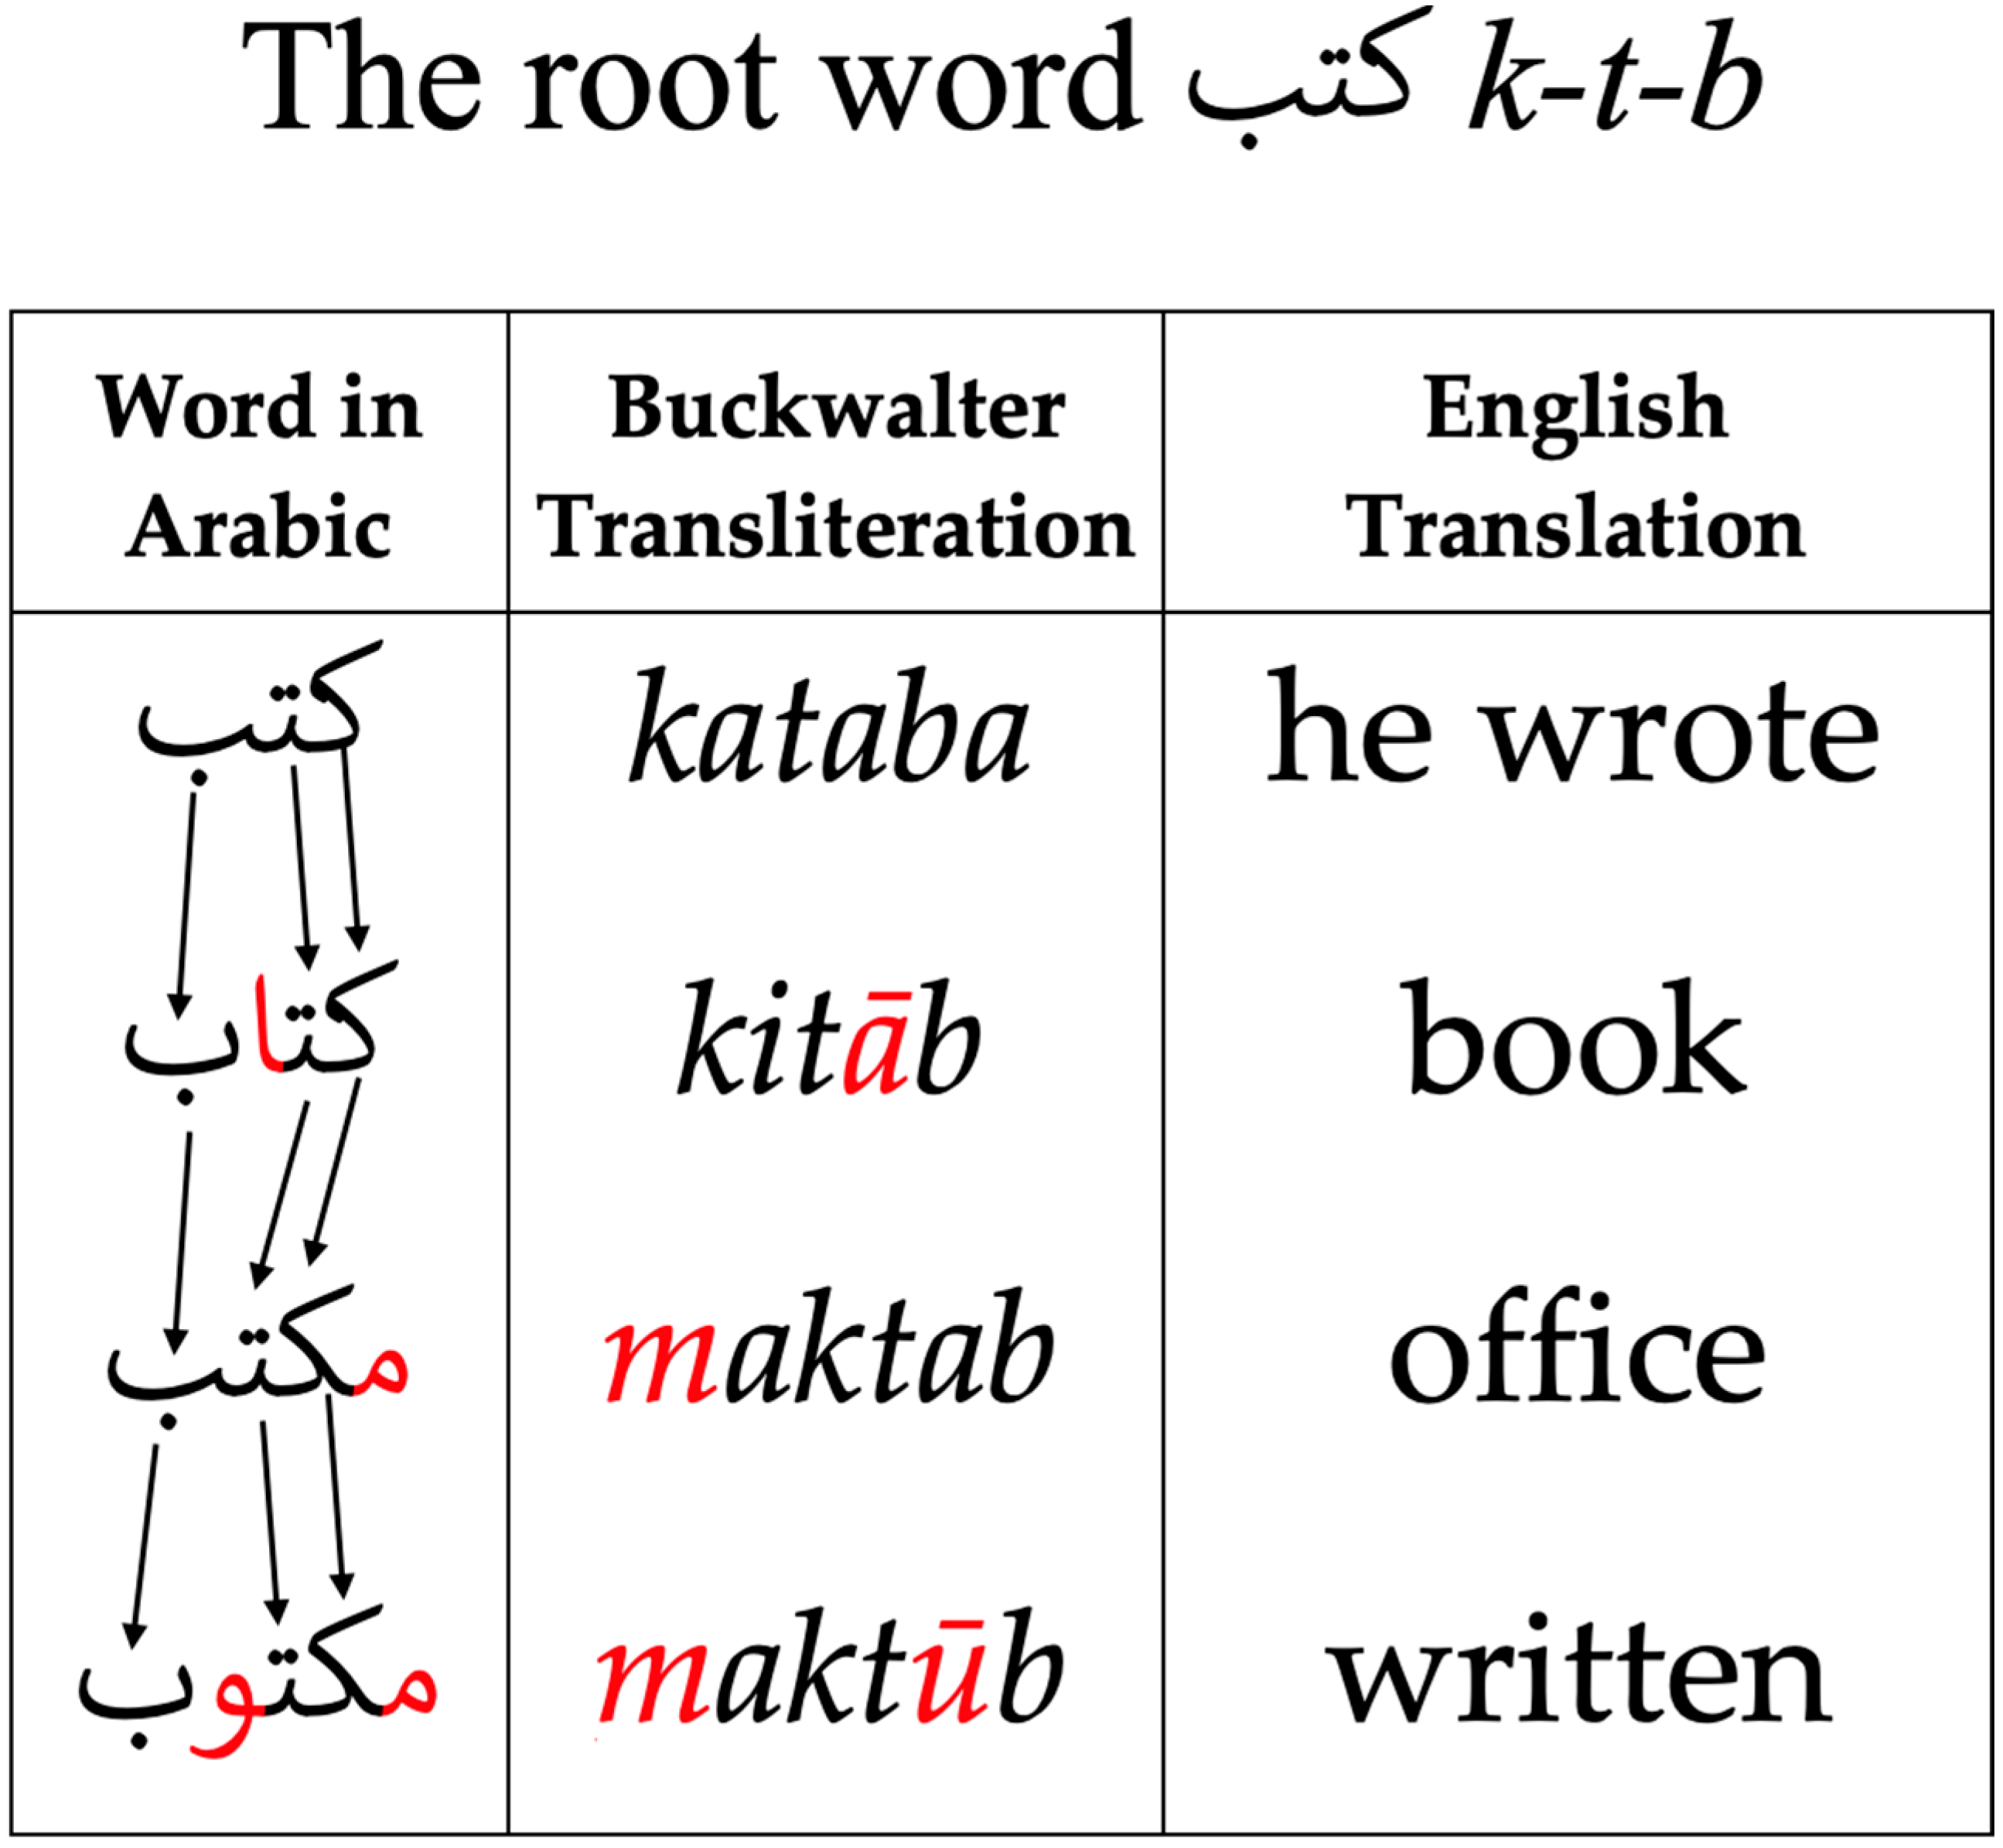
\includegraphics[width=0.72\textwidth]{morphology.png}
\caption{Example of Arabic morphological derivation from the root ``k-t-b'', illustrating the
richness and complexity of Arabic word formation.}
\label{fig:arabic_morphology}
\end{figure}

In addition to root-based derivation, Arabic has extensive \emph{cliticization}: function words
such as the definite article, conjunctions, prepositions and pronouns are written attached to a
host word. For example, the single written token \textit{walfi\d{d}\d{d}a} (``and the silver'')
joins three morphological units: the conjunction \textit{wa+} (``and''), the definite article
\textit{al+} (``the'') and the noun \textit{fi\d{d}\d{d}a} (``silver''). The BAREC annotation
guidelines explicitly name the presence and type of clitics as markers of readability level
\cite{habash2025guidelines}, which is why making them explicit through morphological
segmentation (D3Tok) is central to the methodology of this thesis.

Lexical ambiguity is another challenge, since a single undiacritized Arabic word can correspond
to several readings. The written form \textit{`lm}, for example, can be read as \textit{`ilm}
(``knowledge''), \textit{`alam} (``flag'') or \textit{`allama} (``he taught''), depending on
the context. Ambiguity affects readability directly, because resolving the rarer readings
requires more advanced linguistic knowledge, and the BAREC guidelines place constructions that
need diacritization for disambiguation at the higher readability levels. Arabic syntax also
allows flexible word order, which makes sentences harder for models to analyse.

Finally, Arabic has few large annotated readability resources compared with English. Earlier
Arabic datasets use three to six levels, cover one curriculum, one genre or one learner
population, and are annotated at the level of words or whole documents rather than sentences.
BAREC changed this situation, but fine-grained prediction across 19 ordered levels remains
difficult: two expert annotators agree exactly on only 61.1 per cent of sentences
\cite{elmadani2025barec}.

These challenges lead to two complementary design decisions. First, we use a pretrained
transformer encoder whose contextual representations, learned from large Arabic corpora, help
with the morphological, lexical and syntactic complexity. Second, we use ordinal-aware learning
methods to model the ordered structure of the readability levels, which standard classification
ignores.

\section{Problem Statement}

Readability assessment systems often treat readability prediction as a standard classification
problem trained with cross-entropy. Readability levels, however, are ordered, and nearby levels
are more similar than distant ones. In standard classification, when the true level is 11,
predicting level 10 gets exactly the same penalty as predicting level 1, although the first is
a near miss and the second a far miss.

This thesis therefore investigates the following questions. Given a fixed AraBERTv2 backbone
with D3Tok morphological segmentation and the training protocol of the BAREC benchmark,
\emph{which ordinal head and loss function achieves the highest Quadratic Weighted Kappa (QWK)
among cross-entropy, regression with mean squared error, ordinal log loss, an Earth Mover's
Distance loss, four soft-label settings, a CORAL ordinal head and a two-phase Soft-QWK schedule;
how do the loss families differ in the trade-off between exact-match accuracy and
distance-aware agreement; and are their errors near misses or far misses?} And, as the
contribution that goes beyond the benchmark, \emph{do loss functions developed for readability
in other languages, or named as future work by the BAREC systems, carry over to fine-grained
Arabic readability?}

\subsection{Research Objectives}

The main objectives of this thesis are:
\begin{itemize}
\item Determine which ordinal head and loss function give the highest QWK on the BAREC benchmark
when the corpus, the encoder and the entire training protocol stay fixed.
\item Compare nine head and loss configurations on a single AraBERTv2 and D3Tok backbone, and
report the two-phase Soft-QWK schedule beside them as a separate group.
\item Bring to Arabic three loss functions that have not been evaluated on BAREC: CORN and two
pairwise ranking objectives from readability research in other languages, each compared with
its matched control from the main comparison.
\item Quantify the trade-off between exact-match accuracy (\textit{Acc19}) and distance-aware
agreement (QWK) across the loss families.
\item Measure the error distance of each method, separating near misses from far misses, as the
research topic requires.
\item Establish whether a CORAL head can learn its cut-points under this protocol at all, and
what its cut-points should be initialised to if it cannot.
\item Measure how much of the difference between published systems is due to the checkpoint
selection rule and the decision threshold rather than to the loss.
\item Evaluate predictions at several granularities ($19$, $7$, $5$ and $3$ levels) using the
BAREC collapsing scheme.
\item Compare the results with the original BAREC benchmark, with the systems of the BAREC 2025
Shared Task and with the agreement between human annotators.
\end{itemize}

\subsection{Research Contributions}

The main contributions of this thesis are:
\begin{itemize}
\item A review of Arabic readability work before BAREC, from adapted formulas to lexicons,
curriculum datasets and learner corpora, that identifies what each one could not support and
therefore what a fine-grained sentence-level benchmark adds.
\item A controlled comparison of nine head and loss configurations on one fixed pipeline, which
extends the four losses of the BAREC benchmark with a CORAL ordinal head, four soft-label
settings and a metric-aligned two-phase objective, and reports them in a single table on both
official splits.
\item The first evaluation on BAREC of three losses taken from outside it: CORN, which the ZAI
system paper names as future work \cite{nazzal2025zai}, and the pairwise margin ranking and
pairwise logistic losses used by readability models for Wikipedia in 14 languages
\cite{trokhymovych2024readability} and for English, French and Spanish \cite{lee2022neural}.
\item A verified reproduction of the benchmark's loss comparison, where the one visible
discrepancy is explained and traced back to the checkpoint selection rule.
\item An initialisation of the CORAL cut-points from the cumulative training label frequencies,
motivated by how far the benchmark learning rate lets them travel, paired with a direct
measurement of how much the cut-points actually move and with two ablations that test the
argument from opposite directions.
\item Two metrics of error distance, the share of predictions at least three and at least five
levels away from the gold level. They separate near misses from far misses and show that the
lead in QWK comes from removing far misses and not from lowering the average error.
\item A measurement of how much the checkpoint selection rule and the CORAL decision threshold
are worth, which is what makes systems published under different protocols comparable.
\item A track with a frozen backbone that satisfies the CPU-friendly requirement of the research
topic, reports variance over five seeds and shows that the ranking of the losses on frozen
features does not carry over to fine-tuning.
\end{itemize}

\subsection{Methodology Overview}

The system combines a pretrained transformer language model with ordinal-aware learning
methods. The pipeline is shown in Figure~\ref{fig:pipeline}.

It begins with the BAREC corpus, where each Arabic sentence carries an ordered readability level
from 1 to 19. The input is the D3Tok column of the corpus, a morphologically segmented form in
which clitics are separated from their host word and marked with a \texttt{+}. That
representation is used because AraBERTv2 was pretrained on morphologically segmented Arabic, so
segmented input matches its pretraining distribution, and because the pairing of AraBERTv2 with
D3Tok is the best of the sixteen model and input combinations the benchmark tested
\cite{elmadani2025barec}. The segmented text is tokenised and passed to AraBERTv2, and after
dropout the pooled output of the encoder, a vector of 768 dimensions, is used as the sentence
representation.

This representation goes to a prediction head whose form depends on the configuration. The
softmax losses (cross-entropy, ordinal log loss, EMD and the four soft-label settings) use a
linear layer with 19 outputs; regression, the Soft-QWK schedule and the two pairwise ranking
objectives use a linear layer with a single output; CORAL uses 18 thresholds on one shared
projection; and CORN uses 18 independent binary outputs. During training, the corresponding loss
compares the output of the head with the gold label. At inference, the output is decoded to a
level between 1 and 19 by taking the highest score, by rounding, or by counting how many
thresholds are exceeded. Every configuration is trained and evaluated under the same protocol,
with QWK as the primary metric, together with exact accuracy (\textit{Acc19}), adjacent accuracy
($\pm 1$ \textit{Acc19}), average distance (\textit{Dist}), the collapsed $7$-, $5$- and
$3$-level accuracies, and the two error-distance metrics introduced in this thesis.

\begin{figure}[H]
\centering
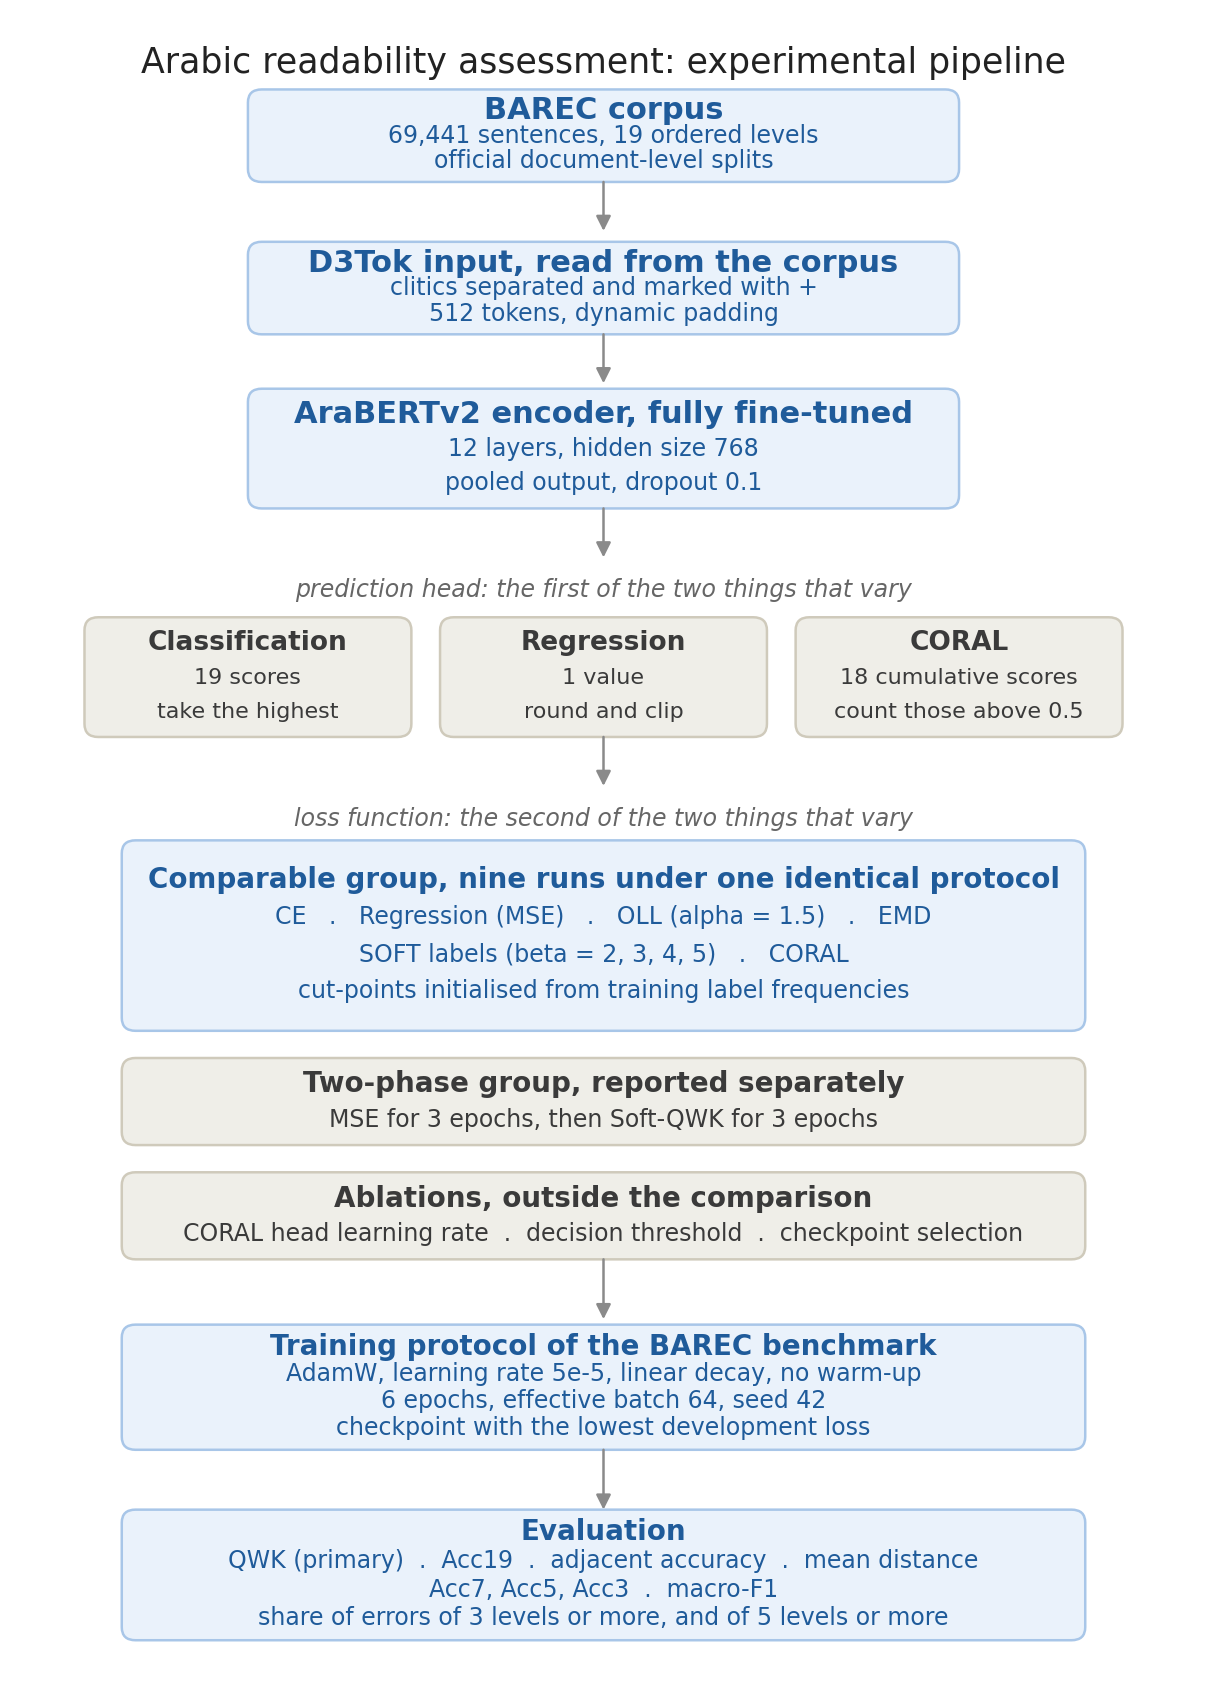
\includegraphics[width=0.78\linewidth]{pipeline.png}
\caption{The experimental pipeline. Everything drawn in blue is held fixed for every run; the
prediction head and the loss function, drawn in grey, are the only components that vary.}
\label{fig:pipeline}
\end{figure}

\subsection{Thesis Organization}

The thesis is organized as follows.
\begin{itemize}
\item \textbf{Chapter 1, Introduction:} the background and motivation, the challenges of Arabic
readability, the research questions, objectives and contributions, and an overview of the
methodology.
\item \textbf{Chapter 2, Literature Review:} readability assessment in general, from formulas to
transformers and to the ordinal and ranking losses used for readability in other languages;
then Arabic readability, the Arabic projects that came before BAREC and what each one could not
support; then the BAREC corpus, the reasons for the D3Tok input and the AraBERTv2 encoder, the
ordinal learning methods, the systems of the BAREC 2025 Shared Task, and where this thesis
stands among them.
\item \textbf{Chapter 3, Proposed Methodology:} the corpus and its splits, the D3Tok input, the
encoder and the prediction heads, the exact form of every loss function with the tests that
verify it, the three added losses, the initialisation of the CORAL cut-points, the training
protocol with every declared difference from the published script, the evaluation metrics and
the frozen-backbone track.
\item \textbf{Chapter 4, Experiments and Results:} the integrity checks, the reproduction of the
published benchmark, the full results on both splits, the trade-off between exact accuracy and
ordinal agreement, the analysis of error distance, the three ablations of the fine-tuning track
and the one of the frozen track, the results of the three added losses, a comparison with
published systems and human agreement, and the limitations.
\item \textbf{Chapter 5, Conclusion and Future Work:} the findings, the contributions, the
limitations and the next steps, the first of which is a study over multiple seeds.
\end{itemize}

\section{Summary of Introduction}

This chapter introduced readability assessment, the particular difficulties of Arabic and the
gap that BAREC filled after two decades of smaller Arabic resources. It stated the research
questions, which ask which ordinal head and loss function gives the highest QWK on BAREC when the
protocol is held fixed, whether the errors are near misses or far misses, and whether losses
from readability research in other languages carry over to Arabic. It listed the nine
configurations of the comparable group, the two-phase Soft-QWK schedule, the three added losses
and the ablations, and described the AraBERTv2 and D3Tok pipeline and the evaluation metrics.

\textit{The next chapter reviews readability assessment in general, then Arabic readability and
the projects that preceded BAREC, and then the BAREC corpus and the methods this thesis builds
on.}
